\chapter{Systemdesign} \chaplabel{systemdesign}

In diesem Kapitel stelle ich die tatsächliche Umsetzung des Projektes vor. Ich
werde auf alle relevanten Designentscheidungen eingehen und erläutern, welche
Alternativen es gab und warum wir welche Methode gewählt haben. Insbesondere
geht es dabei um die Auswahl und Befestigung der Hardwarekomponenten, die
System-Architektur, die unterstützenden Softwarekomponenten sowie die
Verbindungen zwischen den jeweiligen Komponenten.

\section{Sensortypen}

Den Kern der Hardware bilden die Sensoren, die die Bewegungen der Hand
aufzeichnen. Hierfür kommen einige Sensortypen infrage, welche ich nun
vorstellen werde. Dabei werde ich erläutern, warum wir uns in diesem Projekt
für die Verwendung von IMUs entschieden haben.

\subsection{Flex- und Stretchsensoren} \subseclabel{flex}

Viele Forschungsprojekte, die mit Sensorhandschuhen arbeiten, verwenden
Flexsensoren um den Beugungsgrad der Finger oder Fingerglieder zu messen.
Diese Flexsensoren können zum Beispiel aus einem biegsamen elektrischen
Widerstand bestehen, dessen Widerstandswert vom Grad der Biegung abhängig ist.
Mithilfe eines Spannungsteilers kann ein analoges Signal erzeugt werden, dessen
Stärke die Biegung angibt. Alternativ kommen Stretchsensoren (z.B. optische
Linearcodierer) zum Einsatz, welche die Verlängerung eines auf der Oberseite
der Finger gespannten Bandes beim Beugen der Finger messen.

Beide Sensortypen sind zwar sehr einfach zu verwenden, haben jedoch einige
Einschränkungen. So lassen sich Flexsensoren meist nur in eine Richtung biegen
und werden beschädigt, wenn man sie in die falsche Richtung zwingt, und
Stretchsensoren können keine Stauchung messen.

Außerdem liefern sie nur einen eindimensionalen Wert. Die vielen Freiheitsgrade
der Hand zu erkennen würde entsprechend viele dieser Sensoren erfordern. Dies
ist zum einen nicht wünschenswert, da sowohl die Kosten als auch der
Wartungsaufwand hoch wären, zum anderen würden viele Sensoren den Tragekomfort
einschränken und flüssiges Tippen erschweren.

Hinzu kommt, dass Flex- und Stretchsensoren nur einen relativen Wert zu einem
physisch nahen Bezugspunkt angeben können. Man könnte die gesamte Hand mit
Sensoren ausstatten und wäre dann trotzdem nur in der Lage die Handbewegungen,
nicht aber Bewegungen des ganzen Armes über der Tastatur zu erkennen.

Aus diesen Gründen haben wir uns gegen die Verwendung dieser Art von Sensor
entschieden.

\subsection{Visuelles System}

In \secref{visuelles-system} habe ich einige Projekte vorgestellt, in denen
Kamera-Tracking verwendet wird. Dazu wird ein zwei- oder dreidimensionales Bild
der Hände aufgenommen und analysiert. Hierfür kommen komplexe
Bild\-erkennungs\-al\-go\-rith\-men zum Einsatz, um die Position der Hand und
der Finger zu extrahieren.

Wir haben uns aus zweierlei Gründen gegen diesen Ansatz entschieden. Zunächst
ist bereits das Extrahieren der relevanten Daten ein erheblicher Aufwand und
ein schwieriges Problem, sodass wir vermutlich nicht die angestrebte
Genauigkeit erreichen würden. Außerdem haben handelsübliche Kameras eine
Bildrate von \SI{30}{Hz}, sodass wir unsere angestrebte Datenrate damit nicht
erreichen könnten.

Hinzu kommt, dass man hierfür eine Kamera korrekt platzieren müsste und sich
dann nicht aus ihrem Sichtfeld entfernen dürfte. Dies widerspricht unserem
Anspruch, ein von der Haltung und Position unabhängiges und mobiles System zu
entwickeln.

\subsection{Inertial Measurement Units (IMUs)} \subseclabel{imu}

Zuletzt möchte ich die Vorteile von IMUs aufzeigen, welche uns dazu bewegt
haben, diese zu verwenden.

IMUs sind heutzutage als integrierte Schaltungen leicht erhältliche Bausteine
zur Messung kinetischer Eigenschaften. Sie enthalten in der Regel zwei oder
drei MEMS-Bausteine (mikroelektromechanisches System): Das Accelerometer misst
die lineare Beschleunigung, das Gyroskop die Winkelgeschwindigkeit, und das
Magnetometer die Ausrichtung relativ zum Erdmagnetfeld. Üblich sind hierbei
jeweils 3 DoF (\fremdwort{degrees of freedom}, Freiheitsgrade), also Messungen in
jeweils 3 verschiedenene Achsen.

Häufig werden diese IMUs als ,,System-in-Package'' ausgeliefert, das heißt sie
enthalten einen Mikrocontroller, der eine Vorverarbeitung der gemessenen Daten
durchführt und diese, genau wie auch die Rohdaten, über ein geeignetes
Protokoll, zum Beispiel \iic, zur Verfügung stellt. Dabei läuft ein
Fusionsalgorithmus auf dem Chip, der versucht, aus den gemessen Werten die
absolute Orientierung im Raum abzuleiten. Diese wird dann als Euler-Winkel oder
Quaternion\footnote{Die Quaternion ist ein mathematisches Konstrukt, welches
unter anderem für die Repräsentation von Drehungen oder Orientierungen im
dreidimensionalen Raum verwendet werden kann. Sie besteht aus 4 Werten und hat
rechnerisch einige Vorteile gegenüber z.B. Euler-Winkeln.} kodiert
bereitgestellt.

Besonders interessant ist für uns die Unabhängigkeit dieser Sensoren von ihrer
Befestigung. Durch diese sind wir in der Lage, für jeden Finger eine IMU zu
verwenden. Um Fingerbewegungen relativ zur Hand und auch Bewegungen der ganzen
Hand ermitteln zu können, wird zusätzlich eine IMU am Handrücken befestigt.

Wir halten die relative Beschleunigung und die relative Orientierung der Finger
zur Hand für die beiden aussagekräftigsten Messwerte beim Tippen. Diese Werte
erhalten wir mit wenig Aufwand und sowohl in ausreichender Genauigkeit als auch
angemessener Geschwindigkeit von handelsüblichen IMUs.

IMUs haben jedoch auch einige Nachteile. Insbesondere die kostengünstigeren
MEMS-Bausteine sind teilweise ungenau und ihre Daten rauschen mehr oder weniger
stark. In Flugzeugen beispielsweise kommen für die Navigation auch IMUs zum
Einsatz, hier werden dann allerdings hochwertige und sehr teure IMUs verwendet,
die auf anderen Technologien basieren.

Problematisch sind bereits sehr kleine Messfehler. Möchte man anstatt der
Beschleunigung vom Accelerometer die Position des Sensors errechnen, muss man
diese zweimal über die Zeit integrieren (Beschleunigung $\rightarrow$
Geschwindigkeit $\rightarrow$ Position). Eine kleine Abweichung der
Beschleunigung bewirkt von da an eine falsche Geschwindigkeit, sodass die
Position immer weiter abweicht. Um dies zu verhindern, sind möglichst genaue
Daten, gute Kalibrierung, und Fehlerkorrekturschritte nötig, etwa das
Annullieren der Geschwindigkeit zu bekannten Zeitpunkten der Ruhe. Ähnliches
gilt für die Orientierung, da das Gyroskop nur die Rotationsgeschwindigkeit
ermitteln kann -- diese kann jedoch durch Messung des Gravitationsvektors und
des Erdmagnetfeldes besser korrigiert werden.


\section{System-Architektur}

\begin{figure}
    \centering
    \begin{tikzpicture}[
    onslide/.code args={<#1>#2}{%
        \ifdefined\only
        \only<#1>{\pgfkeysalso{#2}}%
        \else
        #2
        \fi
    },
    every node/.style={
        font=\small,
        inner sep=0pt,
        thick,
    },
    node distance=2cm,
    database/.style={
        cylinder,
        shape border rotate=90,
        aspect=0.2,
        draw,
        minimum width=2.5cm,
        text width=2.5cm,
        align=center,
        minimum height=1.5cm,
    },
    node/.style={
        rectangle,
        draw,
        text width=2.5cm,
        align=center,
        minimum height=1cm,
        rounded corners=2pt,
    },
    arrow/.style={
        thick,
        ->,
        >=stealth,
    },
    learning/.style={
        dashed,
    },
    applying/.style={
        very thick,
    },
    radiation/.style={
        decorate,
        decoration={expanding waves,angle=10,segment length=4pt}
    },
    wire/.style={
        % draw=gray,
    },
    sensor/.style={
        node,
        minimum width=5mm,
        minimum height=5mm,
        text width=0,
        draw,
        rectangle,
        rounded corners=0,
    },
    highlight/.style={
        draw=primary,
        color=primary,
        fill=primary!10!white,
    },
    drawhighlight/.style={
        thick,
        draw=primary,
    },
    texthighlight/.style={
        color=primary,
    },
]

    \coordinate (legend) at (6.5, 0.2);
    \draw[thick,wire]           ($ (legend) + (0,    0) $) -- node[at end, right, xshift=0.2cm] {Wire}  ++(0.5, 0);
    \draw[thick,arrow,learning] ($ (legend) + (0, -0.6) $) -- node[at end, right, xshift=0.2cm] {Learn} ++(0.5, 0);
    \draw[thick,arrow,applying] ($ (legend) + (0, -1.2) $) -- node[at end, right, xshift=0.2cm] {Apply} ++(0.5, 0);
    \draw ($ (legend) + (-0.2, 0.3) $) rectangle ++(2, -1.8);

    \node[node]
        (serialparser)
        at (0, 0)
        {Serial Parser};

    \node[node,left=2cm of serialparser]
        (sender)
        {Micro-\\processor};

    \node[sensor,below left=7mm and 0.5cm of sender.south]  (sensor1) {};
    \node[sensor,below=2mm of sensor1] (sensor2) {};
    \node[sensor,below=2mm of sensor2] (sensor3) {};
    \node[sensor,below right=7mm and 0.5cm of sender.south] (sensor4) {};
    \node[sensor,below=2mm of sensor4] (sensor5) {};
    \node[sensor,below=2mm of sensor5] (sensor6) {};

    \node[below=3cm of sender] {Sensors};
    \draw[wire,onslide={<2> drawhighlight}] (sensor1) -| ($ (sender.south) + (-0.2, 0) $);
    \draw[wire,onslide={<2> drawhighlight}] (sensor2) -| ($ (sender.south) + (-0.12, 0) $);
    \draw[wire,onslide={<2> drawhighlight}] (sensor3) -| ($ (sender.south) + (-0.04, 0) $);
    \draw[wire,onslide={<2> drawhighlight}] (sensor4) -| ($ (sender.south) + (0.2, 0) $);
    \draw[wire,onslide={<2> drawhighlight}] (sensor5) -| ($ (sender.south) + (0.12, 0) $);
    \draw[wire,onslide={<2> drawhighlight}] (sensor6) -| ($ (sender.south) + (0.04, 0) $);

    \draw[radiation,onslide={<3> drawhighlight}]
        ([xshift=2mm,yshift=-0.3cm]sender.east) -- node[midway,yshift=-0.6cm,onslide={<3> texthighlight}] {or WiFi} ([xshift=-2mm,yshift=-0.3cm]serialparser.west);

    \draw[very thick,wire,onslide={<3> drawhighlight}]
        ([yshift=0.2cm]sender.east) -- node[midway,yshift=0.3cm,onslide={<3> texthighlight}] {USB} ([yshift=0.2cm]serialparser.west);

    \node[node,right=1cm of serialparser]
        (keyboard)
        {Keyboard\\Listener};

    \node[database]
        (bag)
        at ($ (serialparser) + (1.75, -2) $)
        {ROS Bag};

    \node[node,text width=6cm,onslide={<5> highlight}]
        (preprocessing)
        at ($ (serialparser) + (1.75, -4) $)
        {Preprocessing};

    \node[node, below=1cm of preprocessing.south west,anchor=north west,onslide={<5> highlight}]
        (apply)
        {Apply\\Network};

    \node[database, below=1.5cm of preprocessing.south east,anchor=east,onslide={<5> highlight}]
        (model)
        {Saved Model};

    \node[node, right=1cm of preprocessing,onslide={<5> highlight}]
        (sampling)
        {Sampling};

    \node[node, below=1cm of sampling,onslide={<5> highlight}]
        (learning)
        {Learning};

    \node[node, text width=9.5cm]
        (os)
        at ($ (apply) + (3.5, -2) $)
        {Operating System};

    \draw [arrow,applying] ($ (serialparser) + (-0.5,-0.5) $) -- +(0, -3);
    \draw [arrow,learning] ($ (serialparser) + (0,-0.5) $) -- +(0, -1) -- (bag);
    \draw [arrow,learning] ($ (keyboard) + (0,-0.5) $) -- +(0, -1) -- (bag);
    \draw [arrow,learning] (bag) -- (preprocessing);
    \draw [arrow,applying] ($ (preprocessing) + (-2.25,-0.5) $) -- +(0, -1);
    \draw [arrow,applying] (model) -- (apply);
    \draw [arrow,learning] (preprocessing) -- (sampling);
    \draw [arrow,learning] (sampling) -- (learning);
    \draw [arrow,learning] (learning) -- (model);
    \draw [arrow,applying] ($ (apply) + (-0.5,-0.5) $) -- +(0, -1);

    \draw[dotted,line width=2pt] ($ (serialparser) !.5! (sender) + (0, -1.5) $) -- node[at end] (bottom) {} +(0, -8);
    \draw[dotted,line width=2pt] ($ (serialparser) !.5! (sender) + (0, 1) $) -- +(0, 0.5);

    \node[anchor=north west,right=10mm of bottom,yshift=0.5em] {\large{}\textbf{HOST PC}};
    \node[anchor=north east,left=10mm of bottom,yshift=0.5em] {\large{}\textbf{GLOVE}};

    \ifdefined\setbeamertemplate
        \only<1-4>{
            \node[node, anchor=north west, minimum width=9.6cm, minimum height=3.2cm, fill=white] at (preprocessing.north west) {Machine learning};
        }
    \fi
\end{tikzpicture}

    \caption[Aufbau des Systems]{Aufbau des Systems. Auf der linken Seite sind
    die Hardwarekomponenten im Handschuh, auf der rechten die
    Softwarekomponenten auf dem Host-PC dargestellt. Die Verbindungen geben an,
    wie die Daten durch die Komponenten gereicht werden.

    Es sind 2 Modi dargestellt. Im Lernmodus wird das Modell erstellt und
    zwischengespeichert, im Anwendungsmodus wird dieses verwendet.}
    \figlabel{overview}
\end{figure}

In \figref{overview} zeigen wir die grundlegende Architektur unseres Systems.
Sie beinhaltet alle Komponenten und deren Beziehungen, die
hauptsächlich Datenströme wiederspiegeln. Das gesamte System kann in zwei Modi
betrieben werden. Beim Lernen kommen dabei andere Komponenten zum Einsatz als
bei der Anwendung.

Gemein ist beiden Modi der Prozess der Datenerfassung. Die rohen Sensordaten
und fusionierten Quaternionen werden vom Mikroprozessor aus den Sensoren
extrahiert und an den Host-PC übertragen. Hierfür stehen zwei alternative
Kanäle zur Verfügung (USB oder WLAN). Das Nachrichtenformat wird im
\Secref{uebertragung} genauer betrachtet.  Die übermittelten Nachrichten werden
vom \fremdwort{Serial Parser} interpretiert.

Im Lernmodus wird außerdem jede Tastatureingabe vom Betriebssystem durch den
\fremdwort{Keyboard Listener} abgefangen. Sowohl die Tastatureingaben als auch
die Sensordaten werden dann zum späteren Lernen zwischengespeichert. Das Lernen
besteht aus den Schritten \fremdwort{Preprocessing}, \fremdwort{Sampling} und
dem tatsächlichen \fremdwort{Learning}. Das gelernte Modell wird ebenfalls
gespeichert.

Im Anwendungsmodus benötigen wir keine Tastatureingabe, stattdessen wird diese
generiert. Hierfür werden die erfassten Daten direkt vorverarbeitet, und an
das neuronale Netz weitergegeben (\fremdwort{Apply Network}), welches das zuvor
gelernte Modell geladen hat. Die Ausgaben des Netzes werden dann in das
Betriebssystem als Tastatureingaben eingespeist.

%Das Anwenden eines bereits gelernten Models ist im Vergleich zum Lernen sehr schnell.

\section{Auswahl des IMU-Boards}

\begin{figure}
    \centering
    \fbox{\includegraphics[width=0.5\textwidth]{../common/images/bno055-nano-boards}}
    \imagesource{https://www.tindie.com/products/onehorse/wearable-bno055-nano-board/}
    \caption[Wearable BNO055 Nano Board]{Das Wearable BNO055 Nano Board ist mit \SI{10 x 10}{\milli\meter}
    Größe ein besonders kleines Breakout Board. Es enthält den von uns
    gewählten Sensor BNO055, wir verwenden pro Handschuh 6 dieser Boards.}
    \figlabel{bno}
\end{figure}

Bei der Auswahl der tatsächlichen IMU haben wir uns in erster Linie an der
Größe des Entwicklungsboards orientiert. Einen Eigenbau in SMD-Technologie zu
löten kam für den Prototyp nicht infrage. Stattdessen suchten wir nach einem
,,Breakout Board''\footnote{Breakout Boards sind Platinen, die einen oder
mehrere IC-Bausteine enthalten, und auf denen ausgewählte Pins dieser Bausteine
zum Anlöten zur Verfügung stehen. Häufig enthalten Breakout Boards auch weitere
Sekundärbauteile zur Ansteuerung, etwa Widerstände oder Kondensatoren. Dies
erleichtert die Ansteuerung der ICs und die Entwicklung von Prototypen.},
welches klein genug ist, um es an der Hand zu befestigen und das Tippen nicht
einzuschränken.

Ein möglicher IMU-Typ war die \productname{InvenSense MPU-9150}, welche die
klassische \productname{MPU-6050} sowie einen \productname{AK8975} 3D-Kompass
enthält. Diese IMU ist in vielen verschiedenen Breakout Boards verfügbar,
dadurch sind auch relativ kleine Bauweisen erhältlich\footnote{zum Beispiel
\url{https://new.sparkfun.com/products/13762}, ein Board mit dem Nachfolger
MPU-9250 -- inzwischen wird die MPU-9150 nicht mehr verkauft.}.

Als Alternative haben wir die \productname{Bosch Sensortec BNO055} evaluiert.
Besonders der Formfaktor des \productname{Wearable BNO055 Nano
Board}s\footnote{erhältlich unter
\url{https://www.tindie.com/products/onehorse/wearable-bno055-nano-board/}}
(siehe \figref{bno}) ist
für unseren Anwendungszweck interessant. Dieses Board ist lediglich \SI{10}{mm}
$\times$ \SI{10}{mm} groß und der eingebaute Fusionsalgorithmus verspricht
Datenraten von bis zu \SI{100}{Hz}.

The BNO055 enthält ein 3 DoF 14-bit Accelerometer, ein 3 DoF 16-bit Gyroskop
und ein 3 DoF Magnetometer \citep{bno055-datasheet}. Das Accelerometer lässt
sich konfigurieren auf einen Wertebereich von
\SI{+-2}{g}/\SI{+-4}{g}/\SI{+-8}{g}/\SI{+-16}{g}. Für das Gyroskop stehen
Wertebereiche zwischen \SI{+-125}{\degree\per\second} und
\SI{+-2000}{\degree\per\second} zur Verfügung. Der enthaltene Mikroprozessor
ist ein 32-bit Cortex M0+, auf dem der proprietäre \productname{Bosch
Sensortec} Fusionsalgorithmus vorinstalliert ist.

Dies macht die Ansteuerung des Sensors besonders einfach, da lediglich über
\iic die entsprechenden Datenregister ausgelesen werden müssen. Im Gegensatz
dazu mussten wir bei der MPU-9150 zuerst eine passende Software aufspielen.

Außerdem ist das Breakout Board der BNO055 kleiner und leichter. Für diese
Vorteile haben wir den höheren Preis von ca. \EUR{24,00} statt ca. \EUR{15,00}
für die MPU-9150 in Kauf genommen und in unserem System die BNO055 verwendet.

Hervorzuheben ist bei der BNO055 weiterhin, dass der Fusionsmodus relativ
mächtig ist. Ist die Sensorfusion aktiviert, stellt der enthaltene Prozessor
nicht nur die berechnete Orientierung (wahlweise als Quaternion oder
Euler-Winkel) bereit, sondern ebenfalls den Gravitationsvektor und die
gravitationsbereinigte Beschleunigung (jedoch relativ zum Sensor). Auch die
Gyroskop- und Magnetometerdaten werden bei aktiviertem Fusionsmodus bereinigt.
Hierfür führt die IMU interne Selbsttests und Echtzeitkalibrierungen durch.
Diese sind im Rohdatenmodus leider nicht verfügbar.

\section{Auswahl des Prozessor-Boards}

Auch für die Auswahl des Prozessors ist der Formfaktor relevant. Da wir diesen
jedoch nicht an den Fingern anbringen müssen, sondern am Handgelenk befestigen,
können wir uns auf andere Features konzentrieren.

Wir wählten das \productname{Adafruit Feather M0
WiFi}\footnote{\url{https://www.adafruit.com/product/3010}} (,,Featherboard'')
aus mehreren Gründen~\cite{featherboard}:

\begin{itemize}
    \item Das Board ist mit \SI{6,1}{g} besonders leicht, und mit
        \SI{5,4}{mm} $\times$ \SI{2,3}{mm} auch relativ klein.
    \item Es enthält das \productname{ATWINC1500} WLAN-Modul, und kann somit
        ohne weitere Hardware kabellos mit dem PC verbunden werden.
    \item Der Prozessor (\productname{ATSAMD21G18} / \productname{Cortex M0+})
        hat 6 eingebaute SERCOMs (Bausteine zur seriellen Kommunikation).
        Jeder dieser SERCOMs kann UART, \iic und SPI unterstützen.  Zur
        Verwendung mit der BNO055 benötigen wir 3 dieser Ports (siehe
        \secref{ansteuerung}).
    \item Das Featherboard kann per LiPo-Akku betrieben werden, und taugt
        gleichzeitig als Ladegerät für diesen, wenn es per USB an eine
        Stromversorung angeschlossen ist. Wir haben den Akkubetrieb nicht
        getestet, prinzipiell erlaubt uns aber das Featherboard den einfachen
        Umstieg.
\end{itemize}

Ein paar weitere Merkmale dieses Produktes, welche für unseren Prototyp
vorerst weniger relevant waren, möchte ich ebenfalls aufzeigen:

\begin{itemize}
    \item Der Prozessor ist mit \SI{48}{\mega\hertz} getaktet und bietet mit
        \SI{256}{\kilo\byte} Flash und \SI{32}{\kilo\byte} SRAM großzügig
        Speicher für einfache Anwendungen (im Vergleich hat der
        \productname{Arduino Uno} mit dem \productname{ATmega328P} nur
        \SI{32}{\kilo\byte} Flash und \SI{2}{\kilo\byte} SRAM bei
        \SI{16}{\mega\hertz} Taktrate).
    \item Der Prozessor ist Arduino-kompatibel. Arduino ist eine open-source
        Plattform, welche es vereinfacht, Mikroprozessoren zu programmieren und
        damit deren Verwendung unkompliziert und leicht zugänglich macht.
        Somit ist auch das Featherboard leicht zu programmieren -- ideal für
        einen Prototyp. Der Hersteller Adafruit liefert alle benötigten
        Bibliotheken und eine gute Dokumentation.
    \item Die Entwicklung der Software wird weiterhin durch die gute
        USB-Unterstützung vereinfacht.
    \item Es stehen 20 GPIO Pins zur Verfügung, 8 davon unterstützen PWM.
    \item Der Prozessor und das Featherboard enthalten kein EEPROM, also
        schreibbaren persistenten Speicher. Dieser ist für unsere Anwendung
        jedoch erforderlich, um die WLAN-Zugangsdaten zu speichern. Wir
        müssen daher ein externes EEPROM in die Schaltung einbringen.
\end{itemize}

% Suche nach arduino kompatible board
% Teensy und Feather-M0 Wifi
% Wifi super

\section{Ansteuerung der Sensoren via \iic} \seclabel{ansteuerung}

Die Ansteuerung der gewählten Sensor-Boards erfolgt ausschließlich über den
\iic-Bus. Zwar unterstützt die BNO055 auch die Ansteuerung über UART,
allerdings ist das Break\-out Board nur für \iic konfiguriert. Über den Pin
\texttt{AD0} lässt sich auswählen, auf welcher der 2 möglichen Slave-Adressen
(\texttt{0x28} oder \texttt{0x29}) die BNO055 antwortet.

Um 6 Sensoren des gleichen Typs ansteuern zu können, von denen jeder nur 2
mögliche Adressen annehmen kann, benötigen wir 3 verschiedene Adressräume. Dies
lässt sich entweder durch getrennte Busse oder durch Adress-Translatoren
erzielen.

Wie bereits erwähnt, stehen beim Featherboard 6 SERCOMs zur Verfügung, das
heißt, wir können 3 getrennte Busse aufbauen und mit je einem Prozessor alle
Sensoren einer Hand ansteuern.

Jeder SERCOM kann zur Verwendung mit \iic, UART oder SPI konfiguriert werden.
Dabei stehen für jeden dieser Bausteine (bis auf Ausnahmen) zwei Sätze Pins zur
Verfügung, an denen die serielle Schnittstelle realisiert wird. Die
Softwarebibliothek ermöglicht es, die SERCOMs zu konfigurieren, und für den
jeweiligen Baustein den verwendeten Modus und die Pins festzulegen.

\begin{table}
    \centering
    \newcommand*\circled[1]{\tikz[baseline=(char.base)]{
    \node[shape=circle,draw,minimum width=1.4em,minimum height=1.4em,inner sep=0pt] (char) {#1};}}

\renewcommand{\arraystretch}{1.2}
\begin{tabular}{@{}lrccccrccccrl@{}}
    \toprule
    & \phantom{X} & \multicolumn{4}{c}{Primäre Pads} & \phantom{X} & \multicolumn{4}{c}{Alternative Pads} & \phantom{X} & \\
    \cmidrule{3-6} \cmidrule{8-11}
    SERCOM &
        & 0 & 1 & 2 & 3 &
        & 0 & 1 & 2 & 3 &
        & Standardbelegung \\ \midrule
    0 &
        & 4\textsuperscript{\(\dagger\)}
        & 3
        & 1
        & 0 &
        & \circled{A3}
        & \circled{A4}
        & 8
        & 9 &
        & Serial1 \\
    1 &
        & 11
        & 13
        & 10
        & 12 &
        & \textendash
        & \textendash
        & \textendash
        & \textendash &
        & \\
    2 &
        & 22
        & \textendash
        & 2\textsuperscript{\(\dagger\)}
        & 5 &
        & 4\textsuperscript{\(\dagger\)}
        & 3
        & 1
        & 0 &
        & \\
    3 &
        & 20
        & 21
        & 6\textsuperscript{\(\ast\)}
        & 7\textsuperscript{\(\ast\dagger\)} &
        & \circled{11}
        & \circled{13}
        & 10
        & 12 &
        & Standard-\iic \\
    4 &
        & 22
        & \textendash
        & 23\textsuperscript{\(\ast\)}
        & 24\textsuperscript{\(\ast\)} &
        & A1
        & A2
        & 2\textsuperscript{\(\dagger\)}
        & 5 &
        & SPI \\
    5 &
        & A5\textsuperscript{\(\ast\)}
        & \textendash
        & 6
        & 7\textsuperscript{\(\dagger\)} &
        & \circled{20}
        & \circled{21}
        & \textendash
        & \textendash &
        & Debugging Port\\
    \bottomrule
\end{tabular}

\begin{itemize}[noitemsep]\scriptsize
    \item[$\ast$] müssen als alternative Pads konfiguriert werden
    \item[$\dagger$] Pins 2, 4, 7 und 8 werden intern für das WLAN-Modul
    verwendet.
\end{itemize}

    \caption[SERCOM Pins am Featherboard]{Aus dem Datenblatt des Featherboards
    gewonnene Übersicht der SERCOMs mit ihren verfügbaren Pins. Jeder SERCOM
    kann \iic, UART und SPI-Schnittstellen an verschiedenen Pins bereitstellen.
    Die verfügbaren Kombinationen lassen sich hier ablesen. Unsere gewählten
    Pins sind eingekreist.}
    \tablabel{sercoms}
\end{table}

In \tabref{sercoms} sieht man die möglichen Pins für das Betreiben der SERCOMs.
Für die Verwendung von \iic sind nur Pads 0 und 1 nötig. Bei der Auswahl der
Pins ist zu beachten, dass der gewünschte SERCOM nicht für eine verwendete
Funktion belegt ist, und dass sich die gewählten Pins nicht überschneiden. Wir
haben uns willkürlich aus den möglichen für die hervorgehobe Kombination
entschieden. Wir definieren 3 \iic-Busse, Bus 0 an Pins A3 und A4, Bus 1 an
Pins 11 und 13, und Bus 2 an Pins 20 und 21.

\begin{figure}
    \centering
    \begin{subfigure}[b]{0.6\textwidth}
        \centering
        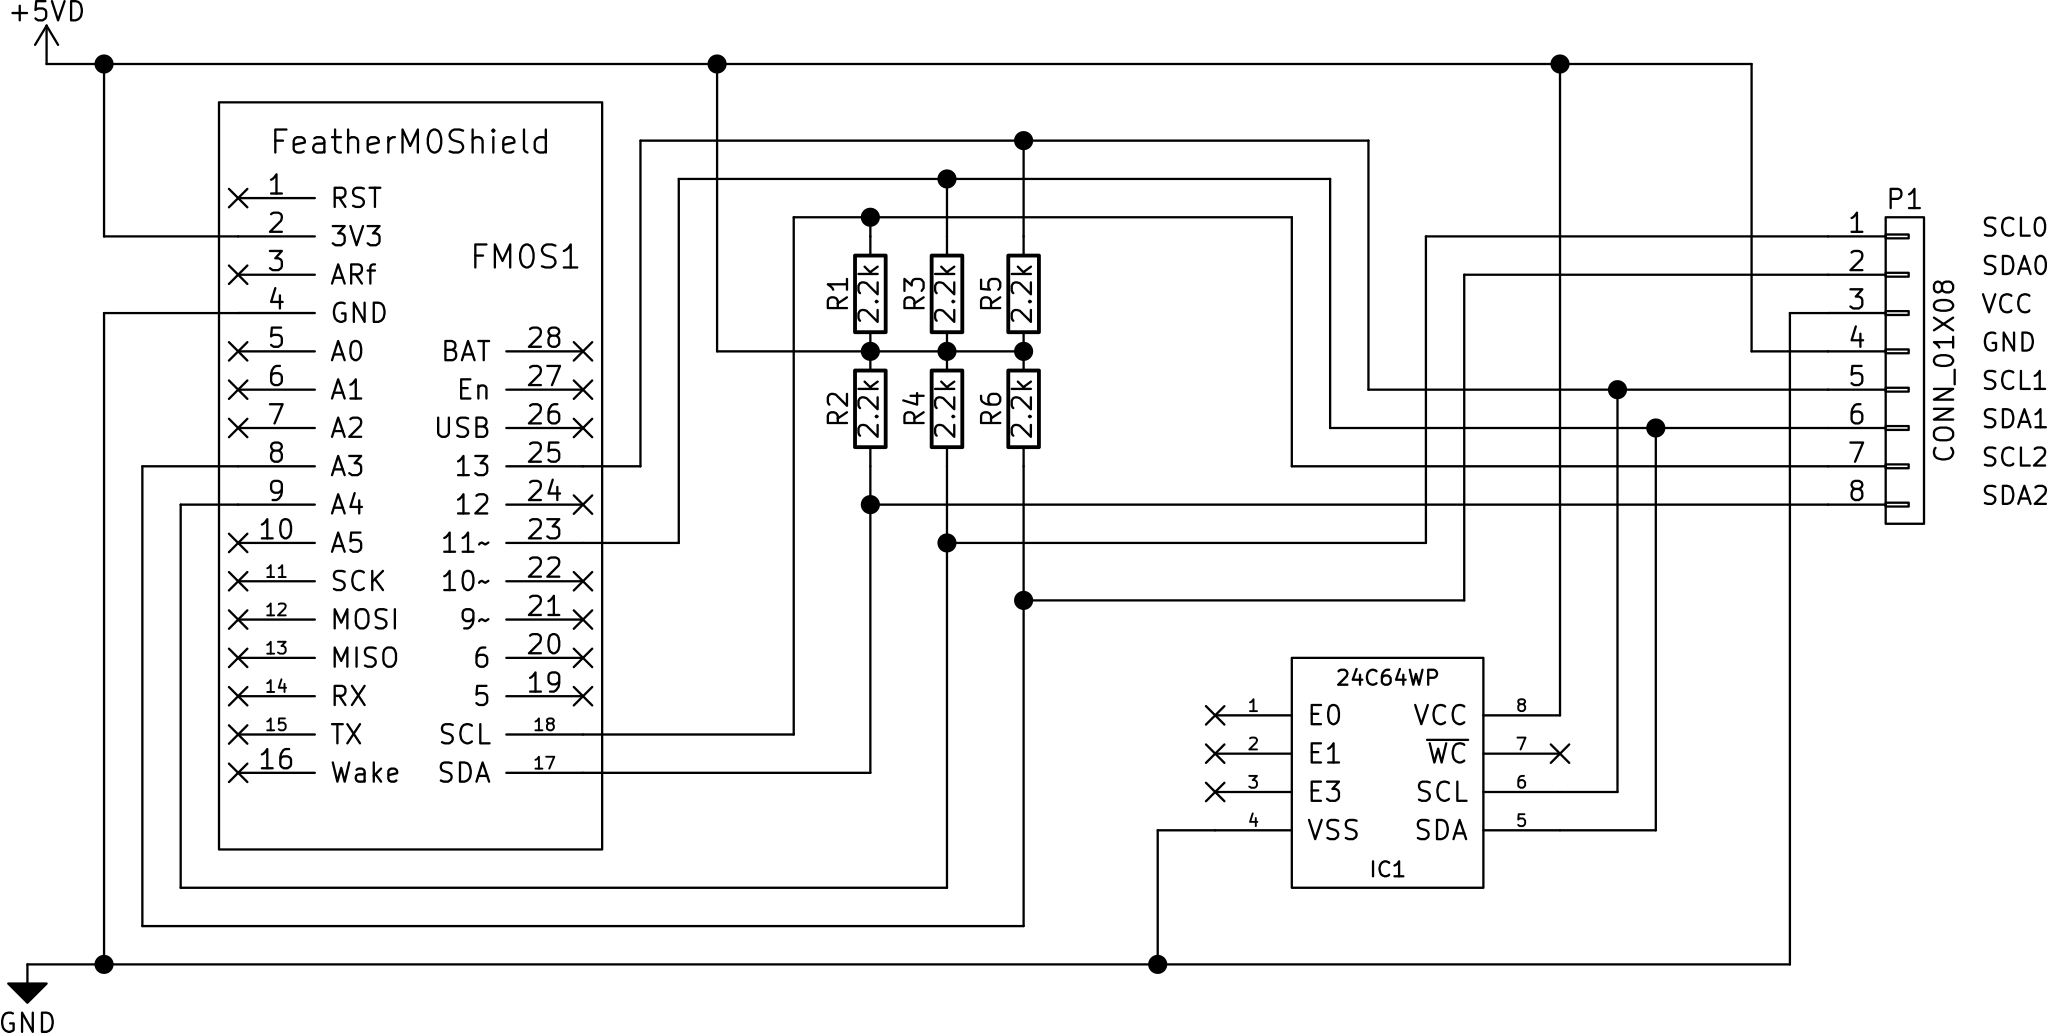
\includegraphics[height=5cm]{../common/images/shield-schematics}
        \caption{Schaltplan}
        \figlabel{shield:schematics}
    \end{subfigure}
    \hfill
    \begin{subfigure}[b]{0.3\textwidth}
        \centering
        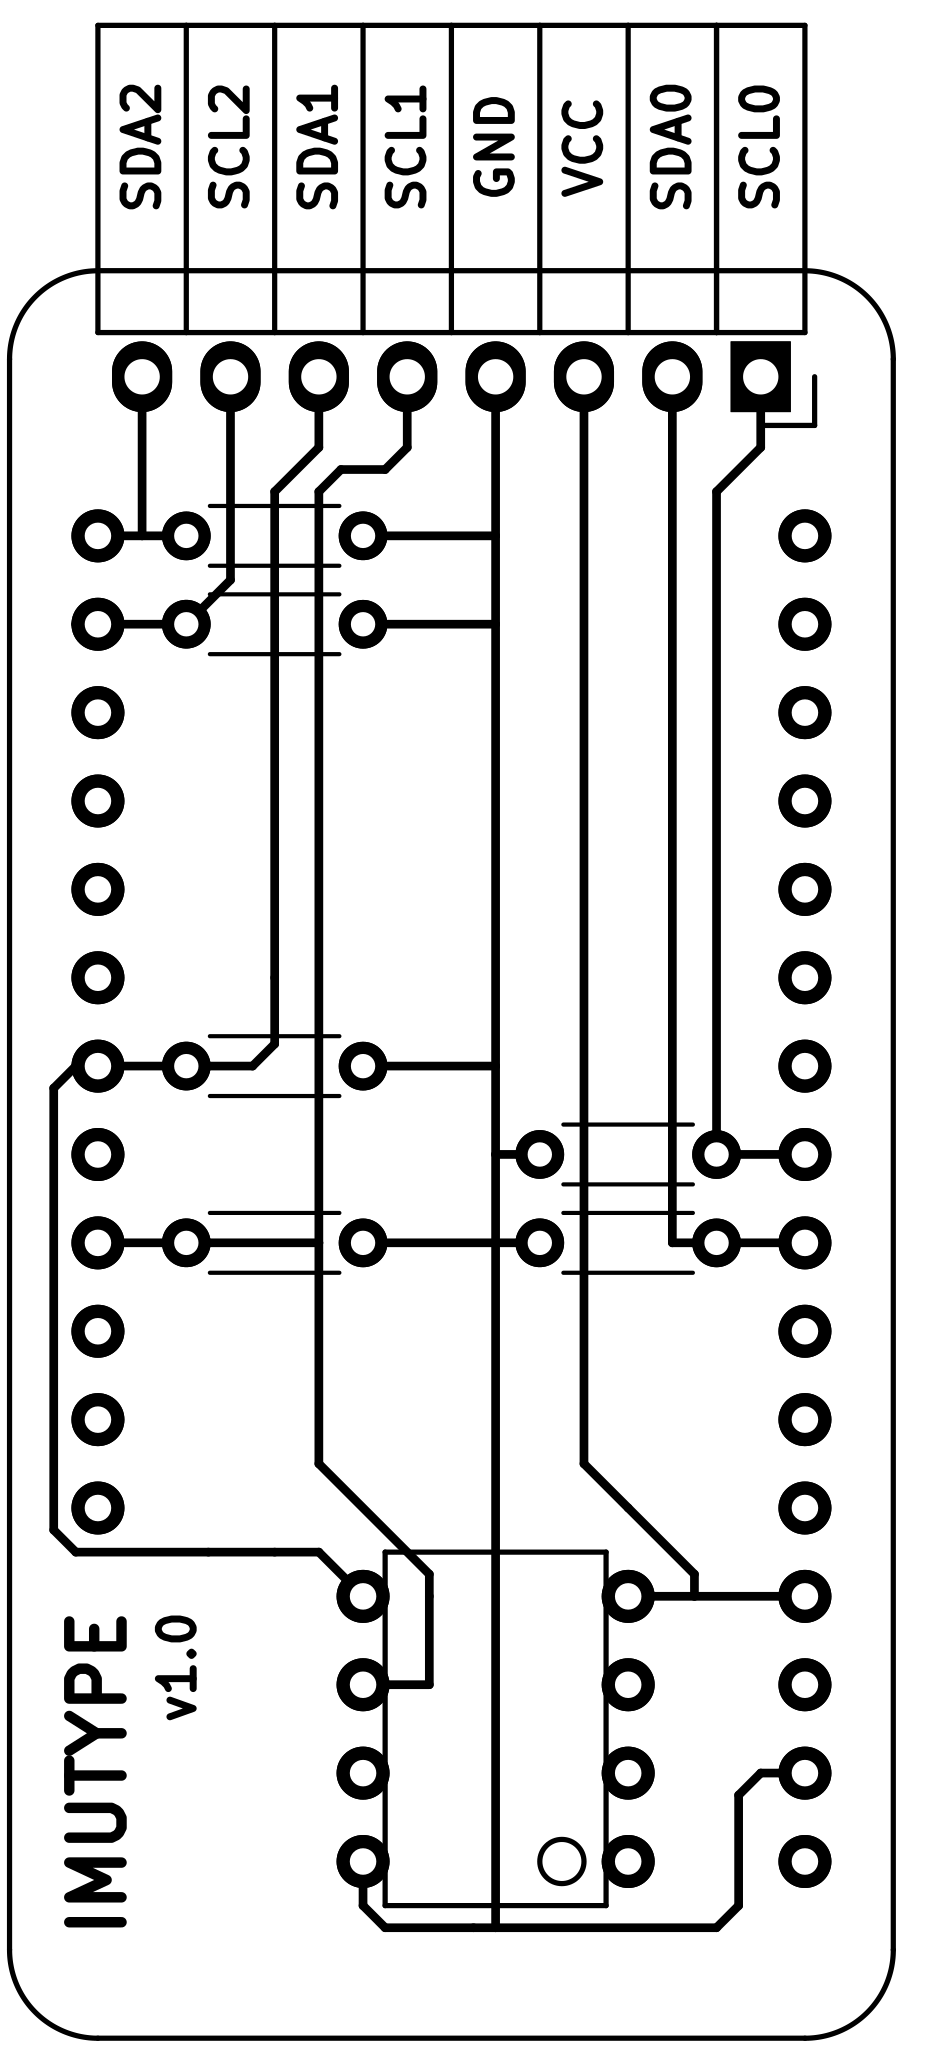
\includegraphics[height=5cm]{../common/images/shield-board}
        \caption{Leiterbahnlayout}
        \figlabel{shield:board}
    \end{subfigure}

    \caption[Schaltplan und Leiterbahnlayout des Shields]{Die Verkabelung der zur Ansteuerung der Sensoren benötigten
    Komponenten erfolgt auf dem ,,Shield'', einer Platine, welche sich auf das
    Featherboard aufstecken lässt (vgl. \figref{photos:shield}).}
    \figlabel{shield}
\end{figure}


In \figref{shield:schematics} sehen wir den Schaltplan für die Verkabelung der
Komponenten am Handgelenk. Nicht enthalten sind die tatsächlichen Sensoren,
diese werden am Ende an die jeweiligen Busse angebracht (VCC, GND, SDA, SCL an
die dazugehörigen Pads auf dem Sensor-Board). Am rechten Rand befindet sich
stattdessen die Buchsenleiste, die SDA und SCL aller Busse sowie VCC und GND
zur Verfügung stellt. Das EEPROM vom Typ \productname{24C64WP} ist an Bus 1
angeschlossen. Zusätzlich enthalten sind die Pull-up-Widerstände, die
erforderlich sind, weil das Featherboard keine integrierten Pull-up-Widerstände
enthält.

Um die Verkabelung einfach zu halten, entwarfen wir einen ,,Shield'' zum
Aufstecken auf das Featherboard. Dieses entspricht dem gezeigten Schaltplan,
und beinhaltet eine Buchsenleiste zum Anstecken des Handschuhs.
\figref{shield:board} zeigt ein mögliches Leiterbahnlayout für diese Schaltung.
Es hat aufgrund der Anordnung der Busse keine Überkreuzungen und benötigt somit
nur eine Kupferschicht. Die Busse sind von links nach rechts in umgekehrter
Reihenfolge angeordnet, dazwischen befinden sich GND und VCC. Die Buchsenleiste
ist ,,oben'', in Handrichtung.

Aus der Anordnung der Busse ergibt sich \tabref{wires}, welche die Zuordnung
der IMUs zu ihrem Bus zeigt, sowie die gewählte Adresskonfiguration. Außerdem
erhält jede IMU eine ID zur späteren Identifizierung der Daten. Auch hier haben
wir darauf geachtet, möglichst wenige Überkreuzungen zu verursachen. Da die
linke und rechte Hand Spiegelbilder sind, aber der gleiche Prozessor und Shield
verwendet werden, haben wir die Reihenfolge der Bus-Zuordnungen umgekehrt. Wie
zu erkennen ist, werden die Busse von rechts nach links an der jeweiligen Hand
angeordnet, statt von innen nach außen.

\begin{table}
    \centering
    \renewcommand{\arraystretch}{1.2}
\begin{tabular}{@{}clllll@{}}
    \toprule
    Hand & IMU & Platzierung & Bus & Adresse & AD0-Pin \\ \midrule
    \multirow{6}{*}{\rotatebox[origin=c]{90}{rechts}} &
      0 & Handrücken        & 2 & 0x28 & low \\
    & 1 & Daumen            & 2 & 0x29 & floating \\
    & 2 & Zeigefinger       & 1 & 0x28 & low \\
    & 3 & Mittelfinger      & 1 & 0x29 & floating \\
    & 4 & Ringfinger        & 0 & 0x28 & low \\
    & 5 & Kleiner Finger    & 0 & 0x29 & floating \\
    \midrule
    \multirow{6}{*}{\rotatebox[origin=c]{90}{links}} &
      6  & Handrücken       & 0 & 0x28 & low \\
    & 7  & Daumen           & 0 & 0x29 & floating \\
    & 8  & Zeigefinger      & 1 & 0x28 & low \\
    & 9  & Mittelfinger     & 1 & 0x29 & floating \\
    & 10 & Ringfinger       & 2 & 0x28 & low \\
    & 11 & Kleiner Finger   & 2 & 0x29 & floating \\
    \bottomrule
\end{tabular}

    \caption{Zuordnung der IMUs zu Positionen an der Hand und den \iic-Bussen
    und "~Adressen.}
    \tablabel{wires}
\end{table}

\section{Befestigung} \seclabel{befestigung}

Besonders für das Ziel der geringen motorischen Einschränkung ist die Wahl der
Befestigungsmethode relevant. Die Testperson muss in der Lage sein, die im
Muskelgedächtnis gespeicherten Bewegungen ohne oder mit nur minimalen
Beeinflussungen auszuführen.

Die Basis-IMU auf dem Handrücken lässt sich am einfachsten auf einem Handschuh
platzieren. Auch vorstellbar ist zum Beispiel ein Clip, welcher sich von der
Handinnenfläche über den Handrücken klemmt. Der erhöhte Produktionsaufwand und
die erschwerte Verkabelung sprachen in unserem Projekt dagegen. Ein schmales
Gummiband um die Hand kam für uns ebenfalls nicht infrage, da dieses stark
gespannt sein müsste, um bei Bewegungen der Hand nicht zu verrutschen, der von
dem Gummiband ausgeübte Druck würde dann jedoch den Tragekomfort
beeinträchtigen.

Besonders wichtig für das Tippen sind die Fingerkuppen, daher haben wir uns
dafür entschieden, diese und das dritte Fingerglied frei zu lassen. Also
befestigen wir die Sensoren am zweiten Fingerglied. Um hier möglichst wenig
Material zwischen die Finger zu bringen, das an den benachbarten Fingern reiben
könnte, nehmen wir ein einfaches Elastikband, und bilden daraus Ringe.  Die
Sensoren kleben wir an der Oberseite auf. Für einen Prototyp ist diese
Konstruktion stabil genug.

% Die an die Testperson angepassten Elastikbänder sind
% zwar so fest, dass sie nicht verrutschen, aber ermöglichen trotzdem noch einen
% hohen Tragekomfort, ohne nach einer längeren Tragzeit abzuschnüren.

Wir verlöteten den \texttt{AD0}-Pin direkt an jedem zweiten Sensor mit
\texttt{GND}. Die vier Kabel leiteten wir am Finger entlang und befestigten sie
mit etwas Faden am fingerlosen Handschuh. So nah an den Fingerspitzen wie
möglich bündelten wir die zusammengehörigen Kabel und verlöteten sie. Dadurch
haben wir die Kabelmenge von 24 auf 8 Kabel reduziert und Gewicht eingespart.
Die 8 übrigen Kabel werden wir zur Steckerleiste geführt, welche auf die
Buchsenleiste des Shields passt. \figref{photos:finished-glove} zeigt den
fertigen Handschuh.

\begin{figure}
    \begin{subfigure}[b]{0.59\textwidth}
        \centering
        \fbox{\includegraphics[height=6cm]{../common/images/glove-sideways}}
        \caption{Der fertige Handschuh}
        \figlabel{photos:finished-glove}
    \end{subfigure}
    \hfill
    \begin{subfigure}[b]{0.4\textwidth}
        \centering
        \fbox{\includegraphics[height=6cm]{../common/images/shield}}
        \caption{Shield und Featherboard}
        \figlabel{photos:shield}
    \end{subfigure}

    \caption[Fotos der Hardwarekomponenten]{Fotos der Hardwarekomponenten.
    Links ist der gesamte Handschuh zu sehen, inklusive der durch Gummiringe an
    den Fingern befestigten IMUs und der Basis-IMU auf dem Handrücken. Der
    Shield ist auf das Featherboard aufgesteckt und durch eine Steckverbindung
    mit dem vorderen Handschuhteil verbunden. Shield und Featherboard (einzeln
    im rechten Bild zu sehen) sind auf einer Manschette am Handgelenk
    befestigt.}
    \figlabel{photos}
\end{figure}

\section{Datenübertragung} \seclabel{uebertragung}

Die erfassten Daten werden vom Mikroprozessor an den Host-PC übertragen. Dies
soll über WLAN, also per Netzwerkprotokoll möglich sein. Zur einfachen
Entwicklung des Systems ist es außerdem wünschenswert, den Handschuh per USB
anzuschließen. Dadurch ist die Verbindung stabil, die Stromversorung
sichergestellt und man muss keine WLAN-Zugangsdaten einpflegen.

Um sowohl die serielle USB-Schnittstelle als auch den netzwerkbasierten Modus
unterstützen zu können, haben wir unser eigenes paketbasiertes Protokoll definiert.
Mithilfe dieses Protokolls können wir die Daten bestimmen, welche übermittelt
werden sollen. Dies hat den Vorteil, dass wir ausschließlich Daten von
Interesse übermitteln und dadurch die Übertragungsgeschindigkeit verbessern.

Paketbasiert bedeutet in unserem Fall, dass wir jede Information in ein
Datenpaket verpacken. Diese werden dann entweder seriell per USB übertragen,
oder unabhängig voneinander per WLAN mit UDP gesendet.

Es gibt in unserem Anwendungsfall 4 verschiedene Arten von Paketen: Header,
IMU Data, Debug Message und Key State Change.

\begin{description}
    \item[Header] Dieses Paket wird immer nach Abschluss des Bootvorganges
        gesendet und beginnt mit einem ,,Magic header'', der willkürlich
        gewählten, festen Bytefolge \texttt{49 D2 C8 CE}. Diese ist hilfreich,
        um zu erkennen, dass es sich tatsächlich um einen Datenstrom vom
        Mikroprozessor handelt. Alle nachfolgenden Bytes auf der seriellen
        Schnittstelle müssen dem in unserem Protokoll formulierten Format
        entsprechen.

        Das Header-Paket beinhaltet die in \tabref{packet-format-header}
        aufgeführten Felder.

        \begin{table}[h]
            \centering
            \begin{tabular}{@{}llll@{}}
                \toprule
                Offset & Länge & Wert & Beschreibung \\ \midrule
                0   & 4 & \texttt{49 D2 C8 CE} & Magic header \\
                4   & 1 & \texttt{03} & Protokollversion \\
                5   & 1 & & Anzahl IMUs \\
                6   & 2 & & Wertebereich Accelerometer \\
                8   & 2 & & Wertebereich Gyroskop \\
                10  & 4 & & Aktuelle Prozessorzeit \\
                14  & 18 & \texttt{00 00 00 \ldots} & Padding auf 32 Byte Länge \\
                \bottomrule
            \end{tabular}
            \caption{Datenformat des Header-Pakets}
            \tablabel{packet-format-header}
        \end{table}

        Die Protokollversion gibt uns die Freiheit, das Protokoll zu erweitern
        und anzupassen, aber mit alten Datensätzen kompatibel zu bleiben.

        Da die Anzahl der IMUs sowie deren Konfiguration hardwareseitig
        festgelegt wird, übertragen wir beides im Header-Paket an den Host,
        sodass dieser die Daten entsprechend korrekt interpretieren kann.
        Ebenso verhält es sich mit den konfigurierten Wertebereichen der
        Sensoren, welche in der späteren Berechnung der tatsächlichen Messwerte
        verwendet werden.
\end{description}

Alle Pakete, die nicht vom Typ Header sind, haben das in \tabref{packet-format}
gezeigte Datenformat.  Die aktuelle Prozessorzeit wird in allen Paketen
übertragen, da es sich um zeitsensible Daten handelt, und die Prozessorzeit die
genaueste Angabe ist, die wir zu einem Datensatz machen können.

\begin{table}[h]
    \centering
    \begin{tabular}{@{}llll@{}}
        \toprule
        Offset & Länge & Wert & Beschreibung \\ \midrule
        0   & 1 & \texttt{C1} & Paketstart-Markierung \\
        1   & 2 & & Pakettyp (s.u.) \\
        2   & 4 & & Aktuelle Prozessorzeit \\
        6 & $l$ & & (Paketinhalt) \\
        $6 + l$ & 1 & \texttt{1C} & Paketende-Markierung \\
        \bottomrule
    \end{tabular}
    \caption{Datenformat aller Pakete, die nicht vom Typ Header sind.}
    \tablabel{packet-format}
\end{table}

Alle Ganzzahl-Werte werden in Little Endian gesendet. Dies ist in
Netz\-werk\-pro\-to\-kol\-len zwar unüblich, da aber die Sensoren die Daten in
dieser Byte-Reihenfolge bereitstellen, ersparen wir uns ein Umsortieren auf dem
Mikroprozessor.

\begin{description}
    \item[Debug Message (\texttt{0x01})]
        Dieser Pakettyp beinhaltet eine Nachricht zur Anzeige auf dem Host, zum
        Zwecke der Entwicklung, um zum Beispiel über die erfolgte Initialisierung
        einer IMU zu informieren. Der Paketinhalt besteht aus 2 Bytes
        Nachrichten-Code (arbiträr), 2 Bytes Textlänge, und dem Text der
        Nachricht, in ASCII codiert.

    \item[IMU Data (\texttt{0x02})]
        Das wohl wichtigste Paket beinhaltet die aktuellen Messwerte einer IMU.
        Der Paketinhalt ist 20 Bytes lang:

        \begin{itemize}[noitemsep]
            \item 6 Bytes lineare Beschleunigung,
            \item 6 Bytes Winkelgeschwindigkeit und
            \item 8 Bytes Orientierung (Quaternion).
        \end{itemize}


        Wir senden keine Fließkommawerte, da die Sensoren Ganzzahlwerte
        bereitstellen, welche unter Berücksichtigung des eingestellten
        Wertebereiches zu Dezimalzahlen in Standardeinheiten umgerechnet werden
        können. Diese Umrechnung findet der Einfachheit halber erst auf dem
        Host-PC statt.  Für die Vektoren errechnet sich der tatsächliche Wert
        durch folgende Formel:

        $$V_{real} = \frac{V_{integer}}{2^{15} \cdot \text{range}}$$

        Den Wertebereich (range) erhält man aus dem Header-Paket.

        Quaternionen sind normalisiert und einheitslos, daher werden sie im
        Gegensatz zu den Vektoren ohne Verwendung eines Wertebereichs
        errechnet:

        $$Q = \frac{Q_{integer}}{2^{14}}$$

    \item[Key State Change (\texttt{0x03})]
        Mit diesem Paket ist der Mikroprozessor in der Lage, eine Taste zu
        simulieren, etwa wenn Buttons am Handschuh befestigt sind. Wir haben
        diese Funktion in anfänglichen Experimenten verwendet, um die
        Funktionalität des Handschuhs zu testen. In Zukunft könnte man
        Funktionstasten in den Handschuh integrieren, etwa um zwischen
        verschiedenen Modi zu wechseln.

        Das Paket beinhaltet neben den üblichen Feldern lediglich einen Key
        Code von 2 Bytes, sowie 1 Byte Tastenzustand (\texttt{0x01} für gedrückt,
        ansonsten \texttt{0x00}).
\end{description}

\section{Datenverarbeitung}

Die Software auf dem Host-PC ist komplett in Python implementiert. Hierfür
kommen hauptsächlich folgende Bibliotheken zum Einsatz:

\begin{itemize}
    \item \texttt{NumPy} \citep{numpy} für die Datenverarbeitung mit Vektoren und
        mehrdimensionalen Matrizen
    \item \texttt{Theano} \citep{theano} und
        \texttt{Lasagne}~\cite{web:lasagne} zur Modellierung und Berechnung der
        neuronalen Netze
    \item \texttt{Matplotlib} \citep{matplotlib} zur Datenanalyse,
        Visualisierung der rohen und vorverarbeiteten Daten, Zeichnen der
        Lernfortschrittsgraphen
    \item \texttt{ROS}~\cite{web:ros} zur Verknüpfung eigenständiger Komponenten über
        wohldefinierte Kommunikationskanäle, sogenannte ,,topics'', dies beinhaltet
        \texttt{rosbag} als Datenspeicher für Lerndaten
\end{itemize}

Die Verwendung von NumPy ist unverzichtbar, da insbesondere
Theano darauf aufbaut. Numpy ist eine weitverbreitete Bibliothek für
die wissenschaftliche Datenverarbeitung in Python. Sie ist einfach zu benutzen,
stark optimiert und auf die Verarbeitung hochdimensionaler Daten ausgelegt.

Theano baut hierauf auf und stellt Funktionen bereit, mit denen
komplexe Rechenoperationen deklariert und dann auf unterschiedliche Arten
ausgeführt werden können. Prinzipiell definiert man mit Theano zuerst den
mathematischen Zusammenhang zwischen verschiedenen Symbolen und lässt sich dann
eine Funktion generieren, welche diese Zusammenhänge auflöst und mitunter sehr
komplexe Berechnungen durchführt. Theano kann konfiguriert werden, diese
Funktion zum Beispiel just-in-time für eine oder mehrere CPUs, oder auch GPUs,
zu kompilieren. Dadurch werden die Berechnungen sehr performant.

Lasagne ist eine Bibliothek, die es vereinfacht, neuronale Netze in Theano zu
modellieren. Dadurch erspart man sich die komplexe Deklaration der
mathematischen Modellierung eines Netzes mit Matrizen, und kombiniert nur
einzelne Netzwerkschichten mit entsprechender Konfiguration zu einem
Gesamtnetz. Dies beschleunigt die Entwicklung extrem und erlaubt es, sehr
flexibel mit der Netzwerkkonfiguration zu experimentieren.

Wir verwenden ROS, das ,,Robot Operating System'' aus verschiedenen Gründen.
ROS ist eine Sammlung von Bibliotheken und Programmen, welche zur Entwicklung
von Robotersystemen in der Forschung dienen. Den Kern bildet hierbei ein
IPC-System (\fremdwort{interprocess communication}), das mithilfe sogenannter
,,topics'' Kommunikation zwischen Prozessen über fest definierte Schnittstellen
erlaubt.

Zunächst benutzten wir diesen Mechanismus der Kommunikation für jeden
Verarbeitungsschritt, etwa auch zwischen Preprocessing und Sampling. Da dies
jedoch einen gewissen Mehraufwand mit sich bringt und Verzögerungen einführt,
entschieden wir uns dazu, nur noch bei einigen Verbindungen ROS-Topics
einzusetzen. Am Ende nutzen wir ROS für die Übermittlung der Rohdaten sowie der
tatsächlichen Tastenanschläge zum Preprocessing, und für die Ausgabe des
Klassifikators im Anwendungsmodus. Alle anderen Verbindungen ersetzten wir
durch Python Koroutinen (\fremdwort{coroutines}), welche ein ähnlich
gekapseltes Programmieren ermöglichen wie die \fremdwort{topic callbacks} von
ROS.

Ein großer Vorteil der Verwendung von ROS für die Rohdaten ist, dass wir
\emph{rosbag} verwenden können. Hierbei handelt es sich um ein Tool, das die
Nachrichten eines oder mehrerer Topics aufzeichnet und später abspielt.
Dadurch konnten wir Lerndaten aufzeichnen, und später mit verschiedenen
Parametern und Algorithmen anhand dieser Daten lernen.  Wir spielen dabei die
Aufzeichnung nicht ab, sondern verwenden die Python-Bibliothek von
rosbag direkt, um die Daten auszulesen.

Es erwies sich als hilfreich, die gesamte Pipeline bis zum Schritt ,,Sampling''
(vgl. \figref{overview}) vom Aufruf des Lernprozesses zu trennen. Das
Zwischenergebnis, ein großes NumPy-Array mit allen Samples, speichern wir in
eine eigene Datei. Wir schrieben uns einige Tools, um diese Samples analysieren
zu können, einige dieser Visualisierungen zeigen wir im \chapref{bewertung}.

Für andere Analysen waren die in ROS enthaltenen Tools sehr hilfreich.
Insbesondere RViz, ein 3D-Visualisierungs-Programm für ROS, ist gut geeignet,
um Fehler bei der Entwicklung zu erkennen. Hauptsächlich nutzte uns RViz beim
Entwickeln der Vorverarbeitung der Quaternionen.

Für die Konfiguration des gesamten Prozesses verwenden wir eine zentrale
Konfigurationsdatei. Diese wird im YAML-Format geschrieben und enthält alle
Parameter, die für den Aufbau des Experiments relevant sind. \lstref{config}
zeigt eine beispielhafte Ausprägung dieser Konfigurationsdatei. Die Bedeutung
der einzelnen Einstellungen wird in \cite{caro} erläutert.  Hervorheben möchte
ich an dieser Stelle, dass wir für jedes Experiment eine eigene
Konfigurationsdatei anlegen können, und somit jedes Experiment nachvollziehbar
und wiederholbar wird. Alle Softwareteile laden beim Start die angegebene
Konfiguration und benutzen die für den jeweiligen Verarbeitungsschritt
relevanten Teile daraus.  Ins jeweilige Verzeichnis des Experiments, neben die
Konfigurationsdatei, werden auch alle Eingabedaten (ROS-Bag),
Zwischenergebnisse (NumPy-Array) und Ausgaben (Lernfortschritt-Statistiken,
generierte Graphen, \ldots) abgespeichert.

\begin{listing}
    \inputminted{yaml}{../common/code/config.yaml}
    \caption[Beispiel für eine Konfigurationsdatei]{Beispiel für eine Konfigurationsdatei. Wir verwenden diese, um die
    Initialisierung aller Softwarekomponenten zu beeinflussen. Dies beinhaltet
    die Vorverarbeitung, die mit Lasagne modellierte Netzwerkarchitektur, das
    Lernverhalten und den Anwendungsmodus.}
    \lstlabel{config}
\end{listing}

\section{Einbindung als Tastatur ins Betriebssystem}

Vorerst unterstützt unser System nur die Einbindung unter GNU/Linux, sodass die
generierten Tastendrücke auch tatsächlich als solche benutzt werden können.
Verwendet wird dafür das Input-Event-System \emph{evdev}, welches über
die dazugehörige Python-Bibliothek sehr einfach zu integrieren ist.

\begin{listing}
    \inputminted{python}{../common/code/evdev.py}
    \caption[Beispiel für die Verwendung von \texttt{python-evdev}]{Beispiel
    für die Verwendung von \texttt{python-evdev} zur Emulation von
    Tastendrücken in einem Linux-System.  Das \texttt{event} stammt hierbei vom
    ROS-Topic \texttt{/predicted\_key\_events}, welches die vom Klassifikator
    erkannten Tastendrücke übermittelt.}
    \lstlabel{evdev}
\end{listing}

Diese Verwendung von \texttt{python-evdev} ist in \lstref{evdev} skizziert.
Eine ähnliche Integration wäre für andere Betriebssysteme selbstverständlich
ebenfalls denkbar.

% vim: tw=79
